\chapter{Theoretical Study and Methodology}\label{ch:3}

\section{System overview}\label{sec:3.1}

\begin{figure}[htbp]
\centering
\resizebox{\ifdim\width>\linewidth\linewidth\else\width\fi}{!}{% Figure 3.1 of report 45 (system architecture), redrawn in TikZ on a fixed grid: Latin Modern text at \small,
% no overlapping labels, no hyphenation inside the boxes. Dashed arrows = knowledge transferred from EchoNext.
\begin{tikzpicture}[font={\footnotesize\hyphenpenalty=10000\exhyphenpenalty=10000}, >={Stealth[length=2mm]},
  box/.style={draw, rounded corners=2pt, align=center, inner sep=3pt, minimum height=1.2cm, text width=#1},
  box/.default=2.4cm, ar/.style={->, thick}, da/.style={->, thick, dashed}]
\node[box=1.6cm, fill=blue!8]    (pdf)  at (0,0)     {ECG printout PDF (vector)};
\node[box, fill=gray!12]         (ras)  at (3.25,2.3)  {Page raster, text removed, grid filtered};
\node[box, fill=gray!12]         (dig)  at (3.25,0)    {Exact vector digitiser (12$\times$2.5\,s + 10\,s)};
\node[box, fill=gray!12]         (med)  at (3.25,-2.3) {Median beat, fiducials, VCG};
\node[box=2.8cm, fill=green!10]  (cnn)  at (6.85,2.3)  {Pixel CNNs: ResNet, ConvNeXt, EfficientNet};
\node[box=2.8cm, fill=green!10]  (fm)   at (6.85,0)    {ECGFounder, ECG-FM, LSTM, \mbox{1-D} ResNet, MiniRocket};
\node[box=2.8cm, fill=green!10]  (feat) at (6.85,-2.3) {LR, LightGBM, ridge EF on 594 features};
\node[box=3.0cm, fill=blue!8]    (en)   at (6.85,4.4) {EchoNext public data in the printout format (pre-training)};
\node[box=1.9cm, fill=orange!14] (ens)  at (10.45,0)   {Nested ensemble / stacking};
\node[box=1.8cm, fill=orange!14] (dec)  at (13.05,0)   {Decision rule: four classes or triage};
\draw[ar] (pdf.east) -- (dig.west);
\draw[ar] (pdf.north) |- (ras.west);
\draw[ar] (dig.south) -- (med.north);
\draw[ar] (ras.east) -- (cnn.west);
\draw[ar] (dig.east) -- (fm.west);
\draw[ar] (med.east) -- (feat.west);
\draw[ar] (cnn.east) -| (ens.north);
\draw[ar] (fm.east) -- (ens.west);
\draw[ar] (feat.east) -| (ens.south);
\draw[ar] (ens.east) -- (dec.west);
\draw[da] (en.south) -- (cnn.north);
\draw[da] (en.east) -| ($(fm.east)+(0.42,0.38)$) -- ($(fm.east)+(0,0.38)$);
\end{tikzpicture}
}
\caption{System architecture of the Phase I pipeline. Dashed arrows: knowledge transferred from the EchoNext public dataset.}\label{fig:3.1}
\end{figure}

The Phase I pipeline (Figure~\ref{fig:3.1}) has three parts. The printout PDF is digitised exactly, turned into image, signal and feature representations, and passed to the model families. External knowledge enters from the public EchoNext data, redrawn in the hospital printout format.

\section{Dataset}\label{sec:3.2}

The data are 1,047 12-lead ECG printouts (PDF) from 993 patients of one tertiary hospital, recorded in 2020--2024. Each page has the standard 3 $\times$ 4 layout (2.5 s per lead), a 10-s lead II rhythm strip, 25 mm/s and 10 mm/mV. Each ECG was matched to an echocardiography report of the same patient, whose EF gives the class. The data were split once by patient into a \textbf{develop-} \textbf{ment set} of 837 ECGs (384 Normal, 185 Mild, 177 Moderate, 91 Severe) used for all modelling and a \textbf{locked test set} of 210 ECGs (96 / 47 / 44 / 23) held back until the final model was frozen.

\section{Exact digitisation and the printout renderer}\label{sec:3.3}

The PDFs are vector drawings: each lead is a polyline of about 700 segments, so the trace is recovered exactly. With the row baselines $y_{\text{base}}$ and column origins $ x_{0}$ of the page,
\EqThreeOne
resampled to 500 Hz. The inverse operation, a \emph{printout renderer}, draws any 12-lead signal on a page identical to the hospital's, rounding each point to whole drawing units as the machine does. Redrawn development ECGs match their real pages: 81 \% of drawn points are identical and the read-back error is 5--13 $\mu$ V.

\section{Input representations and features}\label{sec:3.4}

Four representations were built from each printout:

\begin{itemize}
  \item \textbf{page image}: the waveform area with text removed and the grid filtered, for CNNs;
  \item \textbf{aligned signal}: the 12 leads in their own 2.5-s windows on a common 10-s axis, for ECGFounder and the LSTMs;
  \item \textbf{ECGFounder embeddings}: the 1,024-d final embedding and 150 diagnostic outputs;
  \item \textbf{engineered features}: 594 features, among them 191 clinician-style and vectorcardiographic measurements such as the spatial QRS--T angle, total cosine R-to-T (TCRT) and the QT variability index.
\end{itemize}
\section{Network architectures, preprocessing filters and training}\label{sec:3.5}

\subsection{Preprocessing filters}\label{sec:3.5.1}

\begin{table}[htbp]
\caption{Preprocessing filters and their parameters for each input representation.}\label{tab:3.1}
\small
\begin{tabular}{>{\raggedright\arraybackslash\hspace{0pt}}p{\dimexpr 0.216\linewidth-2\tabcolsep\relax}>{\raggedright\arraybackslash\hspace{0pt}}p{\dimexpr 0.157\linewidth-2\tabcolsep\relax}>{\raggedright\arraybackslash\hspace{0pt}}p{\dimexpr 0.626\linewidth-2\tabcolsep\relax}}
\toprule
\textbf{Input} & \textbf{Step} & \textbf{Filter / operation and parameters} \\
\midrule
Page image (CNNs) & rasterise and crop & vector PDF rendered at 1 px/pt; crop to the waveform area (removes all header text) \\
 & grid removal & colour filter: darkness $=255$ $-$ max$(R, G, B)$ (HSV value); the pink grid has a high value and vanishes \\
 & binarisation & Otsu threshold (clamped) \\
 & denoising & connected components $<6$ px removed (keeps 1-px trace lines that a median filter would erode) \\
 & thickening, resizing & scale-aware dilation; area interpolation to 512 $\times$ 1024, then 256 $\times$ 512 network input \\
 & filter ablations & Gaussian 5 $\times$ 5, $\sigma =1$; median 3 $\times$ 3; bilateral ($ d$ 7, $\sigma$ 50/7); CLAHE (clip 2.0, 8 $\times$ 8 tiles); adaptive Gaussian threshold (block 25, $ C$ 60) \\
\midrule
Digitised signal (ECGFounder) & exact digitisation & vector paths converted at 82 pt/mV and 616$/$3 pt/s; 500 Hz \\
 & power-line notch & IIR notch at 50 Hz, $Q =30$ \\
 & band-pass & 4th-order Butterworth, 0.67--40 Hz, zerophase (forward--backward) \\
 & baseline & 0.4-s moving-median baseline subtracted \\
 & scaling, layout & z-score per lead; 12 leads in their own 2.5-s windows on a 10-s axis (12 $\times$ 5,000) \\
\midrule
LSTM / CNN-LSTM & as above, then decimation & 100 Hz; amplitudes clipped at $\pm5$ mV; 13 signals + 13 mask channels (26 $\times$ 1,000) \\
\midrule
Engineered features & beat analysis & 0.5 Hz high-pass; R-peak detection; Raligned median beats; vectorcardiogram by the Kors matrix \\
\midrule
EchoNext signals & harmonisation & de-normalisation to $\mu$ V; resampling 250 $\rightarrow$ 500 Hz; cascaded median filters (0.2 s, 0.6 s) for baseline removal; clipping; printout cut (2.5-s windows) \\
\midrule
Pixel CNNs (IMG) & page image & waveform area, text removed, grid filtered; 320 $\times$ 640 (ResNet-18) or 384 $\times$ 768 (ConvNeXt-Tiny, EfficientNet-B2); grey channel repeated to RGB \\
\bottomrule
\end{tabular}
\end{table}


Each representation has its own filter chain (Table~\ref{tab:3.1}): a colour filter removes the pink grid from page images, and a 50 Hz notch, a 0.67--40 Hz band-pass and a moving-median baseline filter clean the signals.

\subsection{Network layers and activation functions}\label{sec:3.5.2}

Table~\ref{tab:3.2} gives the layers, kernels, activation functions, normalisation and size of every network. The activation functions used are
\EqThreeTwo
where $\Phi$ is the standard normal distribution function. Every four-class network ends in a softmax; ordinal heads use sigmoids for $ P(y> k)$, and LSTM gates use the sigmoid with a tanh cell activation.

\subsection{Training settings and training accuracy}\label{sec:3.5.3}

Image CNNs were trained with AdamW (learning rate 10$^{-3}$, weight decay 0.05), warm-up and cosine decay, batch 16, up to 30 epochs with early stopping, class-weighted cross-entropy with label smoothing 0.05, weight averaging (EMA 0.99) and augmentation (rotation $\pm2$$^{\circ}$, time and amplitude scaling, translation, random erasing). ECGFounder was fine-tuned with differential learning rates (backbone 10$^{-4}$, head 10$^{-3}$). LSTMs used AdamW (10$^{-3}$), batch 32, gradient clipping and early stopping on inner validation. Table~\ref{tab:3.3} compares training and validation accuracy.

\begin{itemize}
  \item \textbf{Image CNNs} reach 0.52 on training and 0.48--0.52 on validation data: they learn evenly and are not over-fitted.
  \item \textbf{Foundation-feature heads} reach 0.73--0.76 on training folds against 0.51 held out, and fine-tuning drives the training loss to 0.66 while validation loss stays at 1.17. With 837 ECGs for 30.8 million parameters, frozen features, regularisation, nested selection and ensembling were therefore used in all later phases.
\end{itemize}
\subsection{Analysis of transfer learning}\label{sec:3.5.4}

\begin{table}[htbp]
\caption{Layers, activation functions, normalisation and size of every network used in Phase I.}\label{tab:3.2}
\footnotesize\setlength{\tabcolsep}{4pt}
\begin{tabular}{>{\raggedright\arraybackslash\hspace{0pt}}p{\dimexpr 0.172\linewidth-2\tabcolsep\relax}>{\raggedright\arraybackslash\hspace{0pt}}p{\dimexpr 0.440\linewidth-2\tabcolsep\relax}>{\raggedright\arraybackslash\hspace{0pt}}p{\dimexpr 0.111\linewidth-2\tabcolsep\relax}>{\raggedright\arraybackslash\hspace{0pt}}p{\dimexpr 0.155\linewidth-2\tabcolsep\relax}>{\raggedright\arraybackslash\hspace{0pt}}p{\dimexpr 0.119\linewidth-2\tabcolsep\relax}}
\toprule
\textbf{Network} & \textbf{Layers and blocks} & \textbf{Activation} & \textbf{Norm.} & \textbf{Params} \\
\midrule
ResNet-18 & 7 $\times$ 7 conv stem + max-pool; 4 stages $\times$ 2 basic blocks of two 3 $\times$ 3 convs (64--512 channels); global average pool; FC(4) --- 18 weight layers & ReLU & BatchNorm & 11.2 M \\
ECGNet (custom) & 7 $\times$ 7/2 stem; 4 stages of 1--1--2--2 residual SE blocks (widths 64--256) with time-elongated 3 $\times$ 5 kernels; [GAP $\|$ GMP]; dropout 0.3; FC(4) ---13 conv layers & ReLU; sigmoid (SE) & BatchNorm & 6.3 M \\
EfficientNet-B0 & 3 $\times$ 3 stem; 16 MBConv blocks in 7 stages with SE; 1 $\times$ 1 head conv; FC(4) & SiLU & BatchNorm & 4.0 M \\
EfficientNet-B2 (IMG70) & 3 $\times$ 3 stem; 23 MBConv blocks in 7 stages with SE; 1 $\times$ 1 head conv; FC(4) + EF head & SiLU & BatchNorm & 7.7 M \\
MobileNetV3-Large & 3 $\times$ 3 stem; 15 inverted-residual bottlenecks, SE in 8; 1 $\times$ 1 head & h-swish, ReLU & BatchNorm & 4.2 M \\
ConvNeXt-Atto & 4 $\times$ 4 patchify stem; 4 stages of 2--2--6--2 blocks (7 $\times$ 7 depth-wise conv + MLP) & GELU & LayerNorm & 3.4 M \\
ConvNeXt-Tiny (IMG70) & 4 $\times$ 4 patchify stem; 4 stages of 3--3--9--3 blocks (96--768 channels); FC(4) + EF head & GELU & LayerNorm & 27.8 M \\
1-D SE-ResNet & 1-D residual blocks, kernel 9, SE; [GAP $\|$ GMP]; FC(4) & ReLU & BatchNorm & -- \\
ECGFounder (Net1D) & 1-D conv stem (kernel 16, stride 2); 7 stages of 2--2--2--3--3--4--4 blocks (20 blocks; 64--1,024 filters), grouped kernel-16 convs with SE; GAP $\rightarrow$ 1,024-d embedding & Swish & none & 30.8 M \\
MLP head / fusion & dropout 0.5 $\rightarrow$ linear 64 $\rightarrow$ GELU $\rightarrow$ dropout 0.5 $\rightarrow$ linear 4 & GELU & standardised input & 66 k \\
LSTM L0--L4 & 1--2 LSTM layers, 64 hidden units, uni- or bidirectional; [last state $\|$ masked mean]; dropout 0.3; linear 4 & sigmoid, tanh & -- & 18--147 k \\
CNN-LSTM (L5) & 3 $\times$ [Conv1d $ k$ 7, stride 2] (26 $\rightarrow$ 32 $\rightarrow$ 64 $\rightarrow$ 64 channels); BiLSTM-64; linear 4 & GELU; sigmoid, tanh & -- & 117 k \\
Meta-learners & multinomial logistic regression; Frank--Hall ordinal (3 binary logistic models) & softmax; sigmoid & standardised & $<1$ k \\
\bottomrule
\end{tabular}
\end{table}


\begin{table}[htbp]
\caption{Training against validation accuracy of the main networks. Upper part: original project, fixed training/validation split, at the selected epoch (training accuracy is measured during the epoch, with aug- mentation and dropout active). Lower part: frozen-feature models in development cross-validation (repeat 0, seed 42): accuracy on the training folds against the held-out fold.}\label{tab:3.3}
\small
\begin{tabular}{>{\raggedright\arraybackslash\hspace{0pt}}p{\dimexpr 0.343\linewidth-2\tabcolsep\relax}>{\raggedright\arraybackslash\hspace{0pt}}p{\dimexpr 0.156\linewidth-2\tabcolsep\relax}>{\raggedright\arraybackslash\hspace{0pt}}p{\dimexpr 0.151\linewidth-2\tabcolsep\relax}>{\raggedright\arraybackslash\hspace{0pt}}p{\dimexpr 0.164\linewidth-2\tabcolsep\relax}>{\raggedright\arraybackslash\hspace{0pt}}p{\dimexpr 0.184\linewidth-2\tabcolsep\relax}}
\toprule
\textbf{Network} & \textbf{Epochs (selected)} & \textbf{Training accuracy} & \textbf{Validation / held-out accuracy} & \textbf{Train / val loss} \\
\midrule
ResNet-18 (filtered image) & 24 (14) & 0.515 & 0.524 & 1.237 / 1.142 \\
ECGNet (SE-ResNet) & 30 (21) & 0.523 & 0.476 & 1.222 / 1.213 \\
EfficientNet-B0 & 29 (19) & 0.447 & 0.351 & 1.327 / 1.436 \\
$_{-3}$ &  &  &  &  \\
ConvNeXt-Atto (10 ) & 30 (25) & 0.404 & 0.452 & 1.336 / 1.318 \\
1-D SE-ResNet on digitised waveforms & 29 (14) & 0.553 & 0.482 & 1.127 / 1.344 \\
ECGFounder fine-tuned (stages 5--6) & 13 (8) & -- & 0.524 & 0.660 / 1.174 \\
\midrule
ECGFounder linear head (CV) & -- & 0.730 & 0.510 & -- \\
ECGFounder MLP head (CV) & -- & 0.761 & 0.514 & -- \\
Header + ECGFounder MLP fusion (CV) & -- & 0.668 & 0.535 & -- \\
Header + clinical features, logistic regression (CV) & -- & 0.562 & 0.507 & -- \\
\bottomrule
\end{tabular}
\end{table}


\begin{figure}[htbp]
\centering
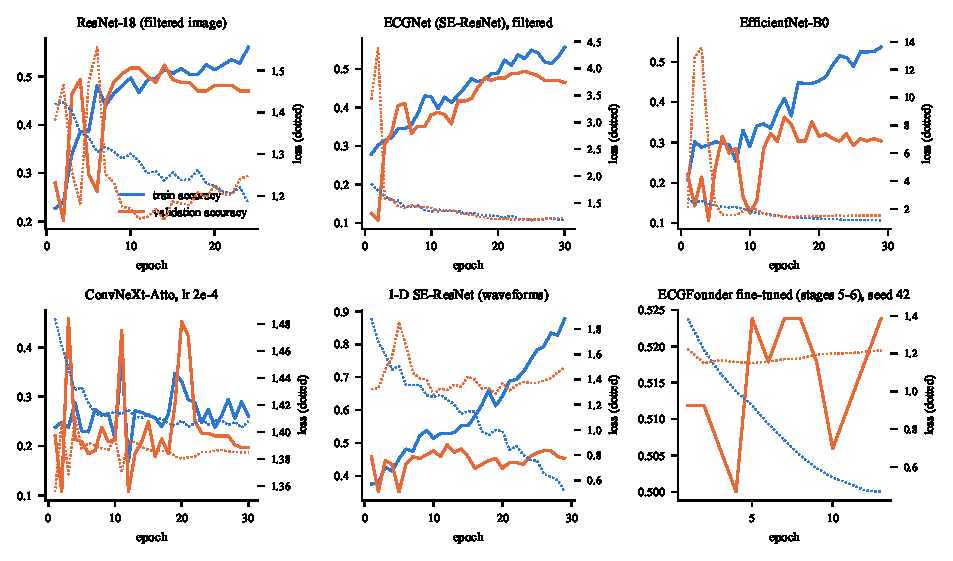
\includegraphics[width=1.00\linewidth,height=0.80\textheight,keepaspectratio]{figures/fig_3_2}
\caption{Training curves of six representative networks: training and validation accuracy (solid) and loss (dotted) per epoch.}\label{fig:3.2}
\end{figure}

\begin{table}[htbp]
\caption{Transfer learning: source, how the knowledge was transferred and what it gave on the hospital printouts.}\label{tab:3.4}
\small
\begin{tabular}{>{\raggedright\arraybackslash\hspace{0pt}}p{\dimexpr 0.199\linewidth-2\tabcolsep\relax}>{\raggedright\arraybackslash\hspace{0pt}}p{\dimexpr 0.295\linewidth-2\tabcolsep\relax}>{\raggedright\arraybackslash\hspace{0pt}}p{\dimexpr 0.505\linewidth-2\tabcolsep\relax}}
\toprule
\textbf{Source} & \textbf{Transfer method} & \textbf{Result on the hospital data} \\
\midrule
ImageNet (1.3 M natural images) & initialise ResNet-18; fine-tune on page images & 0.492 four-class (CV); natural-image features transfer only partly to thin line drawings \\
ECGFounder (10.8 M ECGs, 150 labels) & frozen 1,024-d embedding + linear or MLP head & 0.528--0.542 (CV); screen AUC 0.82; EF $r$ 0.65; best single representation of the project \\
 & partial fine-tuning (stages 5--6; stage 6) & 0.536 (CV); EF $r$ 0.650 against 0.652 frozen: the frozen embedding already holds the EF information \\
 & layer choice (stage 4, 5, 6, diagnostic outputs) & final embedding best (0.544 against 0.517--0.531) \\
EchoNext signals (4,827 US ECG-- echo pairs) & models trained only on EchoNext, applied zero-shot & AUROC 0.85 for EF $\le45$ \%, 0.75 Normal against Mild, EF $ r$ 0.62; four-class 0.551 with no hospital training of the model (only its decision thresholds tuned) \\
 & EchoNext models as stack members & SUPER ensembles 0.583--0.587, the best all-patient results \\
EchoNext images (drawn as printouts) & pre-train pixel CNN, then fine-tune & final ConvNeXt-Tiny ensemble 0.548; ResNet-18: 0.530 against 0.492 with ImageNet only (+3.8 points); EchoNext test accuracy of the pre-trained CNNs 0.58--0.72 \\
\bottomrule
\end{tabular}
\end{table}


Transfer learning was used in four forms, from natural images to EF-labelled ECGs (Table~\ref{tab:3.4}). The closer the source is to the target, the larger the gain: ECG pre-training (ECGFounder) beat ImageNet pre-training by 4--5 points, and EF-labelled public ECGs (EchoNext) supplied the knowledge behind the best ensembles. A model trained only on US patients separates reduced from normal EF on our printouts with AUROC 0.85, which also validates the printout conversion. Frozen ECGFounder features match fine-tuning in EF correlation (0.652 against 0.650) without its over-fitting, and pre-training a pixel CNN on EchoNext ECGs drawn as hospital printouts adds 3.8 points over ImageNet initialisation.

\section{Evaluation protocol}\label{sec:3.6}

\begin{itemize}
  \item \textbf{Cross-validation:} patient-grouped 5-fold CV repeated three times (15 cells), identical folds for every model.
  \item \textbf{Nested choices:} every hyper-parameter, class weight, threshold and ensemble member is chosen inside the training folds \cite{ref37}. Class weights maximise accuracy subject to every recall $\ge0.18$ (fallback 0.15):
\EqThreeThree
  \item \textbf{Intervals and tests:} corrected resampled $t$ statistic \cite{ref38} with Holm adjustment \cite{ref39}:
\EqThreeFour
  \item \textbf{Integrity:} every study was pre-registered in a dated document before it was run; the locked test set was scored once.
\end{itemize}
